%!TEX root=main.tex
\section{背景}
\label{kvdirect:sec:background}


\egg{
\subsection{The Road to High Performance 键值存储}

Building a high performance 键值存储 is a non-trivial exercise of optimizing various software and hardware components in a computer system. The rich literature on 键值存储 performance optimizations can give us a glimpse of software and hardware evolution in recent years.
Early works on distributed in-memory 键值存储 such as Memcached~\cite{fitzpatrick2004distributed} uses OS locks for multi-core synchronization and TCP/IP networking stack for communication. Since then, optimizations have been made on multiple fronts to remove bottlenecks in various parts of the system.


\subsubsection{Synchronization cost}
\label{kvdirect:sec:CoreSynchronizationCost}
Synchronization is needed in multi-threaded 键值存储 implementation since multiple clients might access the same keys concurrently. For example, when two clients make atomic increments to a single key, the value needs to reflect both increments.

To reduce synchronization cost, Masstree~\cite{mao2012cache}, MemC3~\cite{fan2013memc3} and libcuckoo~\cite{li2014algorithmic} optimize caching, hashing and memory allocation algorithms, and replace permissive kernel locks with optimistic version-based locks.
MICA~\cite{lim2014mica, li2016full} takes a further step to completely avoid synchronization by partitioning the hash table to each core so that each core serves an exclusive portion of the hash table.
This approach, however, may introduce core imbalance for long-tail access patterns with a few extremely popular keys~\cite{li2016full}.

\subsubsection{Networking overhead}
\label{kvdirect:sec:ReduceNetworkingOverhead}

In a 键值存储 where computation to communication ratio is low, a significant portion of CPU cycles is spent in the kernel networking stack, including protocol handling, memory copy, system call and multi-core synchronization~\cite{peter2016arrakis}.
Furthermore, the kernel network stack adds hundreds of microseconds latency~\cite{ousterhout2015ramcloud}, which greatly impacts response time.
and complicates latency-hiding programming of applications that require multiple round-trips to the 键值存储.

Extensive research have been done to reduce network communication cost and improve end-to-end latency.
One line of work proposes the 键值存储 server software communicate directly with NICs by polling while bypassing the kernel~\cite{rizzo2012netmap, intel2014data}; packets are processed by a lightweight network stack in user space~\cite{jeong2014mtcp, marinos2014network}.
Chronos~\cite{kapoor2012chronos}, RAMCloud~\cite{ousterhout2010case, ousterhout2015ramcloud} and MICA~\cite{lim2014mica,li2016full} leverage this approach to achieve high throughput (\approx5 million 键值 operations per second (op/s) per core) and low latency (microsecond-scale) by reducing networking overhead.

The other line of work leverage two-sided RDMA~\cite{infiniband2000infiniband} as an RPC mechanism between 键值存储 client and server.
RDMA is a hardware-based transport that almost completely removes the CPU overhead of networking.
键值存储 systems such as HERD~\cite{kalia2014using, kalia2016design} achieve per-core throughput and end-to-end latency comparable or superior to the first line of work, but the overall throughput per server largely depends on the processing capacity of RDMA NIC~\cite{kalia2016design}.

\subsubsection{Throughput bottleneck of CPU}
\label{kvdirect:sec:CPU-键值-Bottleneck}
When pushed to the limit, in high performance 键值存储 systems the throughput bottleneck can be attributed to the computation in 键值 operation and the latency in random memory access. 键值存储 needs to spend CPU cycles for key comparison and hash slot computation. Moreover, 键值存储 hash table is orders of magnitude larger than the CPU cache, therefore the memory access latency is dominated by cache miss latency for practical access patterns.

By our measurement, a 64-byte random read latency for a contemporary computer (Sec.~\ref{kvdirect:sec:evaluation-setup}) is \approx110~ns. A CPU core can issue several memory access instructions concurrently when they fall in the instruction window, limited by the number of load-store units in a core (measured to be 3\approx4 in our CPU)~\cite{gharachorloo1992hiding, han2010packetshader, zhang2015mega}. In our CPU, we measure a max throughput of 29.3M random 64B access per second per core. On the other hand, an operation to access 64-byte 键值 pair typically requires \approx100ns computation or \approx500 instructions, which is too large to fit in the instruction window (measured to be 100\approx200). When interleaved with computation, the performance a CPU core degrades to only 5.5 MOps. An optimization is to batch memory accesses in a 键值 store by clustering the computation for several operations together before issuing the memory access all at once~\cite{li2016full, narula2014phase}. This improves the per-core throughput to 7.9 MOps in our CPU, which is still far less than the throughput of the host DRAM. 
}

\begin{comment}
When pushed to the limit, in high performance 键值存储 systems the throughput bottleneck can be attributed to the computation in 键值 operation and the latency in random memory access. This is actually the bottleneck we want to remove in our design and we discuss the issue here in more detail. 

键值存储 needs to spend CPU cycles for key comparison and hash slot computation. Moreover, 键值存储 hash table is orders of magnitude larger than the CPU cache, therefore the memory access latency is dominated by cache miss latency for practical access patterns.



The latency for CPU to access DRAM on the same NUMA node, \ie cache miss latency, is 80\approx90 nanoseconds on our platform (measured with~\cite{intelmemaccess}, hardware details in sec. \ref{kvdirect:sec:implementation}).
For 64-byte access granularity, the random read latency including data copy is \approx110~ns.
This latency can be partially hidden by the out-of-order execution engine in modern CPUs, which can issue a few memory accesses in parallel.
However, the parallelism is limited by two factors: the number of load-store units (LSUs) per core~\emph{k} (measured to be 3\approx4 on our CPU) and the instruction window size~\emph{W} (measured to be 100\approx200 instructions on our CPU)~\cite{gharachorloo1992hiding, han2010packetshader, zhang2015mega}. When there are enough memory operations in the instruction window, \emph{k} of them can be issued simultaneously. 



Figure~\ref{kvdirect:fig:cpu-mem} shows random memory access performances of a multicore CPU. It shows that a modern CPU core can provide fairly high random memory access throughput (27M~op/s or 1.7~GB/s for 64B granularity). Moreover, memory throughput scales linearly with number of CPU cores, indicating that the DDR main memory is not a bottleneck.

However, in a 键值 store memory access is interleaved with computation for hash slot calculation and key comparison. An operation to access a 64-byte 键值 pair typically requires \approx100 ns computation or \approx500 instructions, which is far larger than the instruction window size.
Consequently, when the random memory access instructions for different keys are separated by computation, the second DRAM access is too far to fit in the same instruction window with the first DRAM access and cannot be issued in parallel.

One can batch memory accesses in a 键值 store, i.e. clustering the computation for several operations together before issuing the memory access all at once~\cite{li2016full, narula2014phase}.
Table~\ref{kvdirect:tab:kv-cpu-throughput} depicts the measured per-core hash table throughput under different 键值 sizes and batch sizes, assuming the 键值 is inlined in hash table and each 键值 operation requires one non-cached memory access.
The results fit the following formulas within 10\% error:
\begin{equation}
%\small
\frac{1}{RandAccessThroughput} = \frac{MemLatency}{Parallelism}
\end{equation}
\begin{equation}
%\small \frac{1}{键值Throughput} = ComputeTime + \frac{MemLatency}{min(BatchSz, Parallelism)}
\begin{aligned}
\frac{1}{键值opThroughput} = & ComputationTime + \\
      & \frac{MemLatency}{min(BatchSize, Parallelism)}
\end{aligned}
\end{equation}
This indicates that when interleaved with computation, the performance of CPU degrades significantly. In the extreme case, even if the instruction window size or memory fetch parallelism goes to infinity, the per-core 键值 operation throughput would still be bounded by computation (\approx10M~op/s), 10\approx20x slower than a single DDR channel.
\end{comment}

\egg{
\subsection{Domain-Specific Architectures for 键值存储}

Ten years ago, processor frequency scaling was over and people turned to multi-core and concurrency~\cite{sutter2005free}.
Nowadays, CMOS feature-size reduction is getting more and more difficult, which implies that multi-core scaling is also over. People are turning to domain-specific architectures (DSAs)~\cite{esmaeilzadeh2013power} for better performance. Several such DSAs have been used to improve 键值存储 performances. 

\egg{
For computation, DSAs such as GPU, 
FPGA~\cite{putnam2014programmable, caulfield2016cloud} and ASIC~\cite{liu2016cambricon, tpu} have been quickly accepted by the market.
For networking, DSAs are also deployed at scale in datacenters, such as RDMA/RoCE NICs~\cite{mellanoxrdma}, programmable NICs~\cite{greenberg2015sdn, li2016clicknp} and programmable switches~\cite{bosshart2013forwarding}.
}

\subsubsection{One-sided RDMA}

Due to high overhead in CPU network processing, DSAs to accelerate networking, such as RDMA/RoCE NICs~\cite{mellanoxrdma}, are deployed at scale in datacenters. High performance 键值存储 systems can leverage RDMA capable hardware. One approach is to accelerate RPC with \textit{two-sided} verbs in RDMA/RoCE NICs (section \ref{kvdirect:sec:ReduceNetworkingOverhead}, Figure~\ref{kvdirect:fig:memaccess-a}).
By doing so, the 键值 performance is bounded by CPU (section \ref{kvdirect:sec:CPU-键值-Bottleneck}).

A significantly different approach is to leverage \textit{one-sided} RDMA to access remote memory via the NIC on the client and bypass the CPU on the server, as shown in Figure~\ref{kvdirect:fig:memaccess-b}.
In this approach, 键值 computation and synchronization are handled by the client CPU, therefore making the 键值 server very light-weight and high performance.
Despite the high message rate (8M\approx150M~op/s~\cite{kalia2016design}) provided by RDMA NICs, it is challenging to find an efficient match between RDMA primitives and key-value operations.
For a write (PUT or atomic) operation, multiple network round-trips and memory accesses may be required to handle hash conflicts, memory allocation and fetch/save non-inline data.
RDMA does not support transactions. Clients must synchronize with each other to ensure consistency by either using RDMA atomics or distributed atomic broadcast~\cite{szepesi2014designing}, both incurring communication overhead and synchronization latency~\cite{mitchell2013using, dragojevic2014farm}.
As a consequence, most RDMA-based 键值存储, \eg, Pilaf~\cite{mitchell2013using}, FaRM~\cite{dragojevic2014farm} and HERD~\cite{kalia2014using} recommend using one-sided RDMA for GET operations only. For PUT operations, they fall back to two-sided RDMA as RPC and let the remote CPU do the actual work. Throughput of write-intensive workload is still bottlenecked by CPU cores.

In addition to the mismatch between RDMA primitives and 键值 operations, implementation of commodity RDMA NICs also constrain 键值 throughput. For example, RDMA NICs hold a lock for atomic operations when a PCIe DMA to the same memory address is in flight, which bounds RDMA atomics throughput to \approx2M~op/s~\cite{kalia2016design}.

\subsubsection{Highly parallel architectures}

Highly parallel architectures such as many-core processors~\cite{berezecki2011many}, GPGPU~\cite{zhang2015mega}.

\subsubsection{FPGA}

FPGA~\cite{istvan2013flexible, chalamalasetti2013fpga, maohardware, lavasani2014fpga, istvan2015hash, istvan2016consensus, kvs-openpower, istvan2015hash, sidler2015scalable, blott2015scaling} have been explored to overcome the limited parallelism of CPU in accessing DRAM.
Compared to general-purpose processors, FPGA has more flexible pipeline parallelism and can be specialized for the key-value store application.
Compared to RDMA, FPGA can support key-value operation primitives directly, as well as specializing network packet format and PCIe DMA operations to use network and PCIe bandwidth efficiently.
Compared to GPGPU, FPGA is more power-efficient and has lower latency.

In recent years, FPGA is becoming cost-effective and is getting deployed at scale in datacenters~\cite{putnam2014programmable, caulfield2016cloud}. Its programmability has been greatly improved~\cite{li2016clicknp}.
Most existing work store the entire hash table inside the on-board DRAM, which is often quite limiting (typically on the order of 4\approx16~GiB), while the host DRAM is often large (on the order of 100\approx500~GiB).
键值-Direct follows this line of work, while leveraging host DRAM for 键值 storage, as depicted in Figure~\ref{kvdirect:fig:memaccess-c}.

键值-Direct leverages a programmable NIC with large-scale deployments in datacenters.
The programmable NIC is composed of two parts: a traditional RDMA NIC plus a field-programmable gate array (FPGA).
There has been research on leveraging the reconfigurability of the NIC for network processing, \eg, network virtualization~\cite{greenberg2015sdn, vfp} and network functions~\cite{li2016clicknp}.
键值-Direct extends the application of programmable NICs to a novel area: key-value stores.
}

\subsection{键值存储 的工作负载变化}
\label{kvdirect:sec:workload-shift}

\textbf{讨论 serverless computing 中的 shared storage}

从历史上看,诸如Memcached \cite {fitzpatrick2004distributed}之类的键值存储作为Web服务的对象缓存系统获得了普及。
在内存计算的时代,键值存储超越了缓存,成为在分布式系统中存储共享数据结构的基础结构服务。
许多数据结构可以在键值哈希表中表示,例如,NoSQL数据库中的数据索引\cite {chang2008bigtable},机器学习中的模型参数\cite {li2014scaling},图形计算中的节点和边缘\cite {shao2013trinity,xiao17tux2}和分布式同步中的序列发生器\cite {kalia2016design,eris}。

工作负载从对象缓存转移到通用数据结构存储意味着键值存储的几个设计目标。

\textbf {小键值的高批量吞吐量。}
内存计算通常以大批量访问小键值对,例如线性回归中的稀疏参数\cite {li2014algorithmic,xiao17tux2}或图遍历中的所有邻居节点 \cite {shao2013trinity},因此键值存储能够受益于批处理和流水线操作。

\textbf {可预测的低延迟。}
对于许多数据并行计算任务,迭代的延迟由最慢的操作决定\cite {ousterhout2015ramcloud}。 因此,控制键值存储的尾部潜伏期非常重要。 由于调度不规则和膨胀缓冲,基于CPU的实现通常在重负载下具有大的波动。
%基于CPU的设计可能需要通过调整批量大小来解决延迟和吞吐量问题 \cite {li2016full},而硬件加速设计可以利用流水线技术提高吞吐量而不会牺牲延迟 \cite {kalia2016design}。
%此外,由于调度不规则,CPU处理时间在高负载下可能会有很大的波动,而硬件流水线通常具有稳定的延迟 \cite {li2016clicknp}。

\textbf {写入密集型工作负载下的高效率。}
对于缓存工作负载,键值存储通常具有比写入更多的读取数量\cite {atikoglu2012workload},但分布式计算工作负载不再是这种情况
例如图形计算\cite {page1999pagerank},参数服务器\cite {li2014scaling}。
对于图表中的PageRank计算\cite {page1999pagerank} 或参数服务器中的梯度下降\cite {li2014scaling},每次迭代读取和写入每个节点或参数一次,并且键值存储将提供相同数量的GET和PUT操作。
序列号发生器(sequencer)\cite {kalia2016design}需要原子增量操作而不需要只读操作。
这些工作负载支持散列表结构,可以有效地处理读写操作。

\textbf {快速原子操作。}
几个非常流行的原子操作出现在应用程序中,例如集中式调度程序\cite {perry2014fastpass},序列号发生器 \cite {kalia2016design,eris},counter \cite {zhu2015packet}和 Web 应用程序中临时值\cite {atikoglu2012workload}。
这需要单个键上的高吞吐量原子操作。

\textbf {支持矢量型操作。}
机器学习和图计算工作负载\cite {li2014scaling,shao2013trinity,xiao17tux2} 通常需要对向量中的每个元素进行操作,
例如,使用标量递增向量中的每个元素或将向量减少为其元素的总和。
没有向量支持的键值存储要求客户端为每个元素发出一个键值存储操作,或者将向量检索回客户端并执行操作。
支持键值存储中的矢量数据类型和操作可以大大减少网络通信和CPU计算开销。

\subsection{高性能键值存储系统的阿基里斯之踵}
\label{kvdirect:sec:state-of-the-art-kvs}

构建高性能键值存储是优化计算机系统中各种软件和硬件组件的重要工作。
键值处理的特点是,最先进的高性能键值存储系统基本上分为三类:
在 键值存储 服务器的 CPU 上
(图~\ref{kvdirect:fig:memaccess-a}),
在 键值存储 客户端上
(图~\ref{kvdirect:fig:memaccess-b})
或者在硬件加速器上
(图~\ref{kvdirect:fig:memaccess-c}).

当推到极限时,在高性能键值存储系统中,吞吐量瓶颈可归因于键值操作中的计算和随机存储器访问中的延迟。
基于CPU的键值存储需要花费CPU周期来进行密钥比较和散列槽计算。
此外,键值存储散列表比CPU高速缓存大几个数量级,因此存储器访问等待时间由实际访问模式的高速缓存未命中等待时间决定。

\begin{figure}[t]
	\centering
	\subfloat[单核。\label{kvdirect:fig:cpu-mem-single}]
	{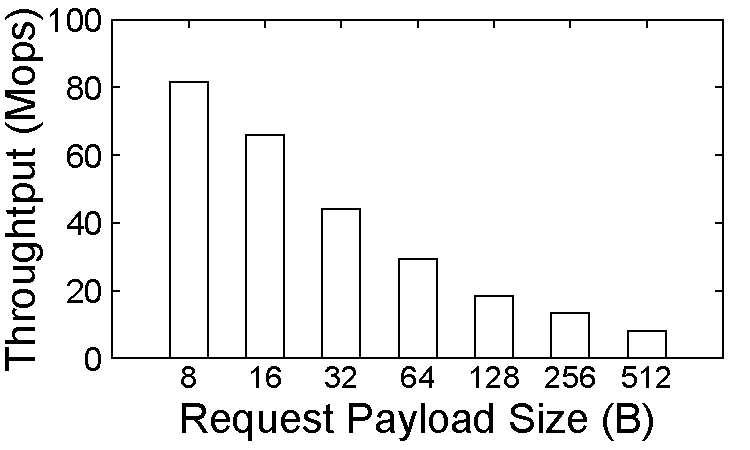
\includegraphics[width=.5\textwidth,page=1]{cpu_random_mem_single_core.pdf}}
	\subfloat[多核。\label{kvdirect:fig:cpu-mem-multi}]
	{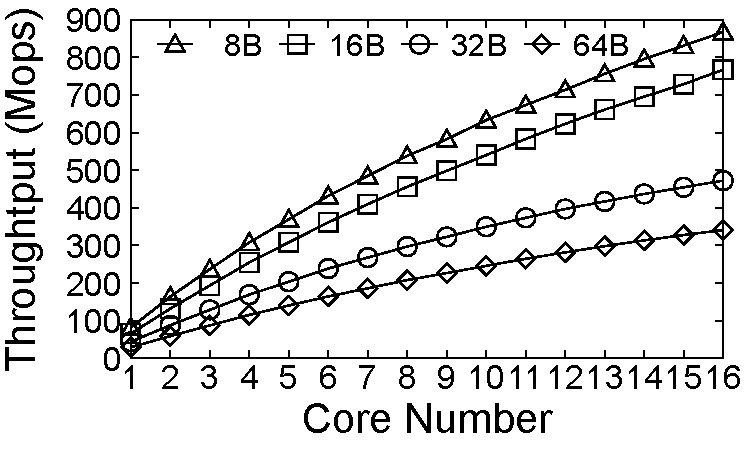
\includegraphics[width=.5\textwidth,page=1]{cpu_random_mem_multi_core.pdf}}
	\caption{CPU 随机内存访问性能。}
	\label{kvdirect:fig:cpu-mem}
\end{figure}

\begin{table}[htbp]
	\small
	\centering
	\label{kvdirect:tab:tput-unroll}
	\begin{tabular}{|c|c|c|c|c|c|c|}
		\hline
		\multirow{2}{*}{大小(字节)} & \multirow{2}{*}{仅计算} & \multirow{2}{*}{仅访存} & \multicolumn{4}{c|}{同时计算和访存(批处理大小)} \\\cline{4-7} 
		&  & & 1 & 2 & 3 & 4 \\\hline
		32 & 24.1 & 44.0 & 7.5 & 11.1 & 13.1 & 14.1 \\\hline
		64 & 11.1 & 29.3 & 5.5 & 6.7 & 7.6 & 7.9 \\\hline
		128 & 5.4 & 18.3 & 3.5 & 4.1 & 4.3 & 4.1 \\\hline
		256 & 2.7 & 13.2 & 2.1 & 2.2 & 2.2 & 2.1 \\\hline
		512 & 1.3 & 8.2 & 1.2 & 1.1 & 1.2 & 1.1 \\\hline
	\end{tabular}
	\caption{不同工作负载和内存访问粒度下的吞吐量(百万次操作每秒)。}
	\label{kvdirect:tab:kv-cpu-throughput}
\end{table}

通过我们的测量,当代计算机的64字节随机读取延迟大约为1~ns。当CPU内核落入指令窗口时,CPU核心可以同时发出多个内存访问指令,受核心中加载存储单元数量的限制(在我们的CPU中测量为3至4个) \cite {gharachorloo1992hiding,han2010packetshader,zhang2015mega}。在我们的CPU中,我们测量每个核心每秒最大吞吐量为29.3~M随机64B访问。另一方面,访问64字节键值对的操作通常需要大约100~ns计算或大约500条指令,这太大而不适合指令窗口(测量为100至200)。当与计算交错时,CPU内核的性能降低到每秒5.5~M 键值操作(Mops)。优化是通过在一次发出内存访问之前将多个操作的计算聚类在一起来批量键值存储中的内存访问\cite {li2016full,narula2014phase}。这将我们CPU中的每核心吞吐量提高到7.9~MOps,这仍远低于主机DRAM的随机64B吞吐量。

观察键值处理中CPU的有限容量,最近的工作是:利用片面RDMA将键值处理卸载到客户端,并有效地将键值存储服务器用作共享内存池。
尽管RDMA网卡提供了高消息率(8 至 150~Mops \cite {kalia2016design}),但要找到RDMA原语和键值操作之间的有效匹配是一项挑战。
对于写入(PUT或原子)操作,可能需要多个网络往返和多个存储器访问来查询散列索引,处理散列冲突并分配可变大小的存储器。
RDMA不支持交易。客户端必须相互同步,以确保使用RDMA原子或分布式原子广播保持一致性 \cite{szepesi2014designing},这两者都会产生通信开销和同步延迟 \cite {mitchell2013using,dragojevic2014farm}。
因此,大多数基于RDMA的键值存储 \cite {mitchell2013using,dragojevic2014farm,kalia2014using}建议仅使用单面RDMA进行GET操作。对于PUT操作,它们会回退到服务器CPU。写入密集型工作负载的吞吐量仍然是CPU核心的瓶颈。

\subsection{FPGA 可编程网卡}
\label{kvdirect:sec:programmable-nic}

十年前,处理器频率扩展速度放慢,人们转向多核和并发\cite {sutter2005free}。
如今,功率上限意味着多核扩展也遇到了困难\cite {esmaeilzadeh2013power}。
人们现在转向领域定制架构(DSA)以获得更好的性能。

%On the spectrum of hardware programmability and performance, general-purpose processors lie on the programmability end, while application-specific integrated circuits (ASICs) lie on the performance end.
%Field-programmable gate array (FPGA) is an architecture between the two extremes, providing both programmability and performance~\cite{bacon2013fpga}.
%As its name indicates, FPGA is a sea of gates.
%Millions of reconfigurable gates and thousands of small block RAMs (BRAMs) provide massive parallelism to build thousands of ``cores'' running simultaneously, and more importantly, customized interconnections among the ``cores'' and BRAMs specializing communication and synchronization for a certain application.
%Consequently, for applications with sufficient bit-level and task-level parallelism, FPGAs provide not only high throughput and power efficiency, but also low and predictable latency.

由于网络速度和CPU网络处理能力的不匹配日益增加,带有FPGA的可编程NIC \cite {vfp,greenberg2015sdn,li2016clicknp,caulfield2016cloud} 现在可以在数据中心进行大规模部署。
如图\ref {kvdirect:fig:kvdirect-arch}所示,我们使用的可编程网卡的核心是FPGA,带有嵌入式网卡芯片以连接到网络。
可编程NIC通常带有板载DRAM作为数据包缓冲区和用于NIC固件的运行时内存\cite {li2016clicknp},但DRAM通常不足以容纳整个键值存储。

\subsection{远程直接键值访问面临的挑战}
\label{kvdirect:sec:challenge}

\begin{figure}[t]
\centering
\subfloat[DMA 吞吐量。\label{kvdirect:fig:dma-tput}]
{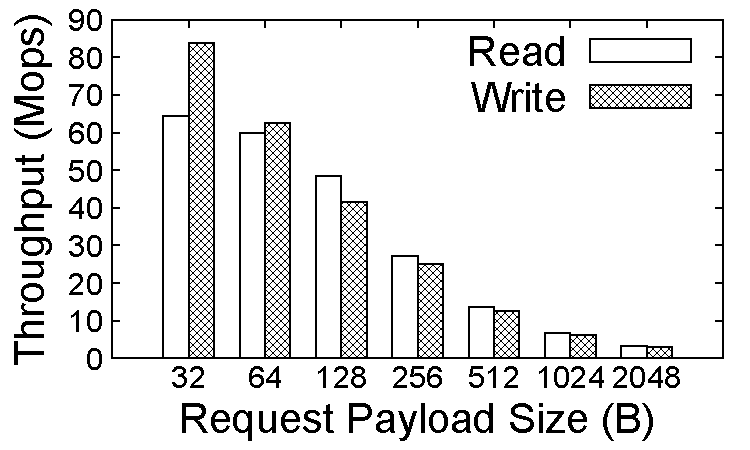
\includegraphics[width=.5\textwidth,page=1]{pcie_bw.pdf}}
\subfloat[DMA 读延迟。\label{kvdirect:fig:dma-lat}]
{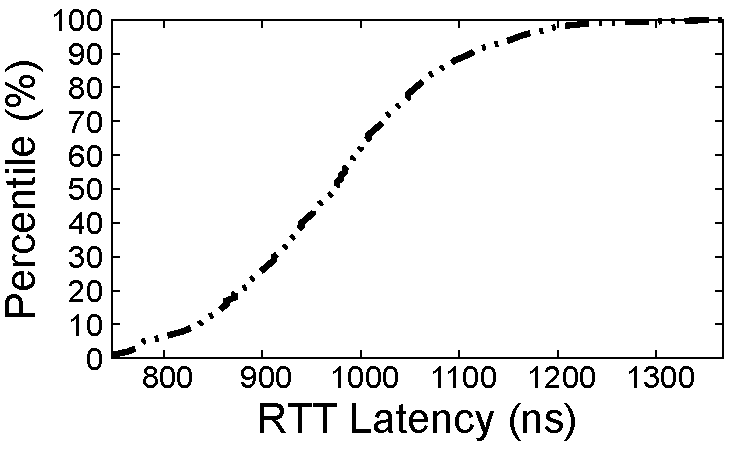
\includegraphics[width=.5\textwidth,page=1]{pcie_latency.pdf}}
\caption{PCIe 随机 DMA 性能。}
\label{kvdirect:fig:dma-perf}

\end{figure}

键值-Direct将键值处理从CPU移动到服务器中的可编程NIC(图\ref {kvdirect:fig:memaccess-c})。
与RDMA相同,键值-Direct NIC通过PCIe访问主机内存。 PCIe是一种分组交换网络,具有大约500 ns的往返延迟和每Gen3 x8端点7.87~GB / s的理论带宽。
在延迟方面,对于我们的可编程NIC,由于FPGA中的额外处理延迟,缓存的PCIe DMA读取延迟为800~ns。
对于随机非缓存DMA读取,由于DRAM访问,DRAM刷新和PCIe DMA引擎中的PCIe响应重新排序,存在额外的250~ns平均延迟(图\ref {kvdirect:fig:dma-lat})。
在吞吐量方面,每个DMA读或写操作都需要一个带有26字节头的PCIe传输层数据包(TLP)和用于64位寻址的填充。
对于以64字节粒度访问主机内存的PCIe Gen3 x8 NIC,理论吞吐量因此为5.6~GB / s或87~Mops。

为了使用64字节DMA请求使PCIe Gen3 x8饱和,考虑到我们的1050~ns的延迟,需要92个并发DMA请求。
实际上,有两个因素进一步限制了DMA请求的并发性。
首先,基于PCIe信用的流量控制限制了每种DMA类型的飞行中请求的数量。我们服务器中的PCIe根联合体为DMA读取通告了88个TLP发布的头部信用,为DMA读取通告了84个TLP非发布的头部信用。
其次,DMA读取需要分配唯一的PCIe标记来识别可能无序的DMA响应。
我们FPGA中的DMA引擎仅支持64个PCIe标签,进一步将我们的DMA读取并发限制为64个请求,这使得吞吐量达到60~Mops,如图\ref {kvdirect:fig:dma-tput}所示。
另一方面,对于40~Gbps网络和64字节键值对,客户端批处理的吞吐量上限为78~Mops。
为了通过GET操作使网络饱和,NIC上的键值存储必须充分利用PCIe带宽,并且每个GET实现接近一个平均内存访问。
这归结为三个挑战:

\textbf {最小化每键值操作的DMA请求。}
散列表和内存分配是键值存储中需要随机内存访问的两个主要组件。
以前的工作建议哈希表\cite {dragojevic2014farm,breslow2016horton},即使在高负载因子下,每个GET操作也有接近1个内存访问。
但是,在高于50%的负载因子下,这些表平均每个PUT操作需要多次存储器访问,且方差很大。
这不仅会消耗PCIe吞吐量,还会导致写入密集型工作负载的延迟变化。

除了哈希表查找之外,还需要动态内存分配来存储无法在哈希表中内联的可变长度键值。
最小化每个键值操作的哈希表查找和每个内存分配的内存访问对于在写密集型小键值工作负载下匹配PCIe和网络吞吐量至关重要。

\textbf {隐藏PCIe延迟,同时保持一致性。}
NIC上的高效键值存储必须管理键值操作和DMA请求以隐藏PCIe延迟。
但是,键值操作可能具有依赖性。
在同一个键上的PUT之后的GET需要返回更新的值。
两个相邻的原子添加操作需要在执行第二个之前等待第一个完成。
这需要跟踪正在处理的键值操作并在数据危险时停止管道,或者更好地设计无序执行器以解决数据依赖性而不明确地停止管道。


\textbf {在NIC DRAM和主机内存之间分配负载。}
一个显而易见的想法是使用NIC上的DRAM作为主机内存的缓存,但在我们的NIC中,DRAM吞吐量(12.8~GB / s)与两个PCIe Gen3 x8端点的可实现吞吐量(13.2~GB / s)相当。 
更期望在DRAM和主机存储器之间分配存储器访问以便利用它们的两个带宽。
然而,与主机存储器(64~GiB)相比,板载DRAM很小(4~GiB),需要混合缓存和负载调度方法。

在下文中,我们将介绍键值-Direct,这是一种基于FPGA的新型键值存储,可满足上述所有目标,并描述我们如何应对这些挑战。
